\documentclass[a4paper, notitlepage, 12pt]{scrartcl}
\author{Lukas Rost \\ \small{Teilnahme-ID: 48125}}
\title{Aufgabe 2 \\ \glqq Dreiecksbeziehungen\grqq  - Dokumentation}
\subtitle{37. Bundeswettbewerb Informatik 2018/19 - 2. Runde \\~\\}
\date{29. April 2019}
\usepackage[ngerman]{babel}
\usepackage[utf8]{inputenc}
\usepackage{graphicx}
\usepackage{wrapfig}
\usepackage{color}
\usepackage[dvipsnames]{xcolor}
\usepackage[hidelinks]{hyperref}
\usepackage[top=2.5cm, bottom=1.5cm, left=2.5cm, right=2.5cm]{geometry}
\usepackage{fancyvrb}
\usepackage{caption}
\usepackage{mathtools}
\usepackage{amssymb}
\usepackage{gensymb}
\usepackage{fancyhdr}
\usepackage{lastpage}
\usepackage{svg}

\usepackage{fontspec}
\usepackage{microtype}

\usepackage{tikz}
\usetikzlibrary{patterns}

\usepackage{tabu}
\usepackage{longtable}

\usepackage{minted}
\fvset{breaklines=true}

\usepackage[framemethod=tikz]{mdframed}
\newmdtheoremenv{kasten}{Beobachtung}

\pagestyle{fancy}
\lhead{Lukas Rost, Teilnahme-ID: 48125}
\rhead{Aufgabe 2, Seite \thepage ~von \pageref{LastPage}}
\cfoot{ }

\newenvironment{longlisting}{\captionsetup{type=listing}}{}

\newmintedfile{cpp}{frame=single,linenos,samepage=false,firstnumber=1,rulecolor=\color{Gray},autogobble,breakafter=.,fontsize=\small}

\begin{document}
\renewcommand{\contentsname}{\centerline{Inhaltsverzeichnis}}
 \maketitle
 \tableofcontents
 \thispagestyle{empty}
 \newpage
 \setcounter{page}{1}
 
 \section{Lösungsidee}
 \subsection{Mathematische Präzisierung der Aufgabenstellung}
 Bei der Eingabe handelt es sich um eine Menge $D = \{d_1,...,d_n\}$ von Dreiecken $d_i$. Jedes Dreieck ist dabei durch seine drei Eckpunkte vollständig definiert ($d_i = \{p_1,p_2,p_3\}$). Ein Eckpunkt ist dabei wiederum ein Punkt $p_i = (x_i,y_i)$ des $\mathbb{R}^2$. \\ \\
 Die Aufgabenstellung fordert nun, dass eine Abbildung $D' = f(D)$ gefunden werden soll. Diese ordnet der Menge $D$ eine Bildmenge $D'$ zu. Für diese müssen bestimmte Bedingungen gelten:
 \begin{itemize}
 	\item Für jedes $d \in D'$ gilt:
 	\begin{equation}
 	\forall ~(x,y) \in d: y \geq 0 \wedge x \geq 0
 	\end{equation}
 	Alle Punkte müssen also über oder auf der x-Achse sowie rechts oder auf der y-Achse liegen.
 	\item Für jedes $d \in D'$ gilt:
 	\begin{equation}
 	\exists ~(x,y) \in d: y = 0
 	\end{equation}
 	Es muss also in jedem Dreieck mindestens einen Punkt geben, der auf der x-Achse liegt. Die Menge aller solchen Punkte eines Dreiecks sei $N_i$ (anschaulich die Menge der Straßenecken). 	
 	\item Jedes $d'_i \in D'$ muss kongruent zum entsprechenden $d_i \in D$ sein. Genauer gesagt muss $d'_i$ aus $d_i$ durch eine Abfolge von Kongruenzabbildungen, d.h. Translationen, Rotationen und senkrechten Achsenspiegelungen\footnote{ und Spiegelungen an einem Punkt, wobei man diese jedoch auch durch Rotationen um $180\degree$ erreichen kann. Demzufolge müssen sie nicht betrachtet werden.} hervorgehen.
 	\item Für jedes $d \in D'$ und jedes $e \in D'$ gilt:
 	\begin{equation}
 	d \cap e = \emptyset
 	\end{equation}
 	$d \cap e$ stellt dabei die Schnittfläche der beiden Dreiecke dar. Es dürfen sich also keine zwei Dreiecke überlappen.\\ \\
 	Eine Dreiecksanordnung wird als \textbf{erlaubt} bezeichnet, wenn sie diese Bedingungen erfüllt. Die Menge der erlaubten Dreiecksanordnungen sei dabei $E$.
  \end{itemize}
Nun ist eine Dreiecksanordnung $D'$ gesucht, die \textbf{optimal} ist. Eine optimale Dreiecksanordnung sei dabei folgendermaßen definiert:
\begin{itemize}
	\item $D'$ minimiert den folgenden Wert über alle erlaubten Dreiecksanordnungen $E$:
	\begin{equation}
	\max_{d_i \in D' ~ d_j \in D'} \min_{n \in N_i ~ m \in N_j} | n.x - m.x |
	\end{equation}
	Der Minimums-Term bildet dabei den Abstand zwischen zwei Dreiecken als minimalen Abstand der Straßenecken, während der Maximums-Term den maximalen solchen Abstand berechnet.
\end{itemize}
 Die (möglichst) optimale Dreiecksanordnung $D'$ bildet die Ausgabe des Algorithmus, der $f(D)$ möglichst effizient berechnen soll.
 \subsection{Wahl eines geeigneten Algorithmus}
 Die Aufgabe ähnelt einem Packproblem aus der algorithmischen Geometrie. Bei diesen muss man Objekte (z.B. Flächen wie Dreiecke) möglichst dicht in gegebene Container (z.B. ebenfalls Flächen) packen, ohne dass sich die Objekte überlappen.\cite{Src:pack} In der hier gegebenen Aufgabe hat man jedoch zusätzliche Nebenbedingungen, die im vorherigen Abschnitt schon erläutert worden sind. Außerdem muss nicht die eingenommene Gesamtfläche minimiert werden, sondern ein Abstand auf der x-Achse. \\ \\
 Leider sind jedoch fast alle Packprobleme NP-vollständig, sodass auch hier die Annahme nahe liegt, dass dies der Fall ist. Demzufolge stellt sich die Frage, wie man ein solches Problem möglichst so lösen kann, dass man ein Gleichgewicht zwischen Effizienz (d.h. Laufzeit) des Algorithmus und Optimalität der Lösung einstellt. Dafür gibt es verschiedene Herangehensweisen:
 \begin{itemize}
 	\item \textbf{Brute Force und Backtracking:} Bei Brute Force werden einfach alle möglichen Lösungen durchprobiert, während man bei Backtracking eine Lösung schrittweise aufbaut und Schritte wieder zurücknimmt, wenn sie zu keiner zulässigen Gesamtlösung mehr führen können. Beide Ansätze sind in diesem Fall nicht geeignet, da der Lösungsraum extrem groß ist, d.h. es gibt sehr viele mögliche Lösungen. Wenn man Laufzeiten wie $\mathcal{O}(n! \cdot 6^n)$ vermeiden will, die sich durch Beachtung aller Permutationen und Rotationen ergeben, sollte man diese Lösungsansätze also nicht verwenden.
 	\item \textbf{Metaheuristiken:} Zu diesen zählt beispielsweise Simulated Annealing, bei dem man die möglichen Lösungen nach einem globalen Maximum bzw. Minimum einer Bewertungsfunktion absucht. Die Bewertungsfunktion wäre in diesem Fall der Gesamtabstand. Außerdem braucht man für Simulated Annealing eine Möglichkeit, aus einer Lösung eine Nachbarlösung zu generieren, was man in diesem Fall durch z.B. Rotationen der Dreiecke erreichen könnte. Da dies jedoch schwierig zu implementieren ist und man schlimmstenfalls genauso viele Lösungen wie bei Brute Force betrachtet, sind solche Heuristiken ebenfalls nicht geeignet. Auch kann man nicht verhindern, mögliche Lösungen doppelt zu betrachten, was für die Laufzeit ebenfalls nicht so gut ist.
 	\item \textbf{Dynamic Programming oder Greedy-Ansätze:} DP- und Greedy-Algorithmen sind zwar meistens laufzeiteffizient, jedoch nicht immer optimal. Aus diesem Grund sind sie für eine optimale Lösung dieses Problems nicht geeignet. Beispielsweise könnte die von einem Greedy-Algorithmus getroffene Entscheidung für den besten Folgezustand, also z.B. die Platzierung eines Dreiecks, zu einem nicht optimalen Gesamtergebnis führen. Es könnte dann beispielsweise nicht mehr möglich sein, andere Dreiecke dicht an das aktuelle anzulegen, wodurch der Gesamtabstand erhöht würde.
 	\item \textbf{Heuristiken und Approximationsalgorithmen:} Bei Heuristiken versucht man durch intelligentes Raten\footnote{Auf Englisch übrigens auch als \textit{ansatz} bekannt.} und zusätzliche Annahmen über die optimale Lösung zu einer guten Lösung zu gelangen. Eine speziell an das Problem angepasste Heuristik ist für dieses Problem das Mittel der Wahl. Dadurch kann man sowohl eine gute (also polynomielle oder pseudopolynomielle) Laufzeit als auch eine Lösung, die relativ nah am Optimum liegt, erreichen. Eine heuristische Herangehensweise an dieses Problem wird in den folgenden Abschnitten näher beschrieben.
 \end{itemize}
  \subsection{Beschreibung der Lösungsidee}
  \subsubsection{Beobachtungen bezüglich einer guten Lösung}  
  Da ein Dreieck sowohl durch seine Seitenlängen als auch durch seine Innenwinkel charakterisiert wird, scheint es sinnvoll zu sein, diese erst einmal zu berechnen. Sei nun $\varphi_i$ der kleinste Innenwinkel des Dreiecks $d_i$. Der Punkt des Dreiecks, an dem der Winkel anliegt, werde als \textbf{Optimalpunkt} bezeichnet. Ist die Summe $\sum_{i=1}^{n} \varphi_i \leq 180\degree$, dann ist eine optimale Lösung des Problems sehr leicht ersichtlich:
  \begin{kasten}
  	In diesem Fall genügt es, alle Dreiecke so zu platzieren, dass alle einen festen Punkt gemeinsam haben (dieser ist mit dem jeweiligen Optimalpunkt identisch) und sie um diesen herum halbkreisförmig angeordnet sind (siehe Abbildung). Dann ist der Gesamtabstand $0$, da sich alle Dreiecke einen Punkt teilen. Dieser Abstand muss optimal sein, da kein geringerer Abstand als $0$ möglich ist. \\
  	{\centering
  		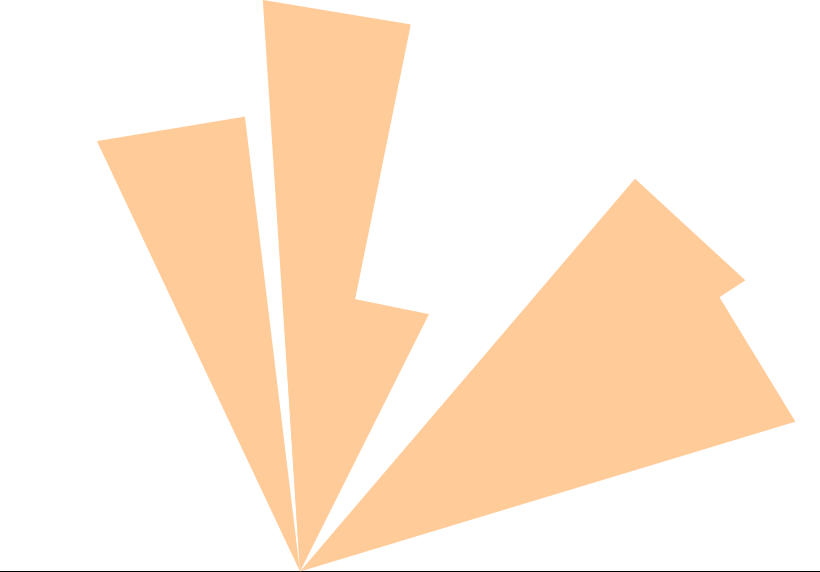
\includegraphics[width=0.6\textwidth]{pics/optimal-tri.png}
  		\captionof{figure}{Optimale Anordnung für eine Summe kleiner gleich $180\degree$}
  	\par}
  \end{kasten} ~\\
 Sollte die Summe jedoch größer sein, ist es nicht mehr so einfach, eine optimale Lösung zu finden. Genauer gesagt kann man ab diesem Punkt nur noch eine Heuristik einsetzen, die ein möglichst gutes Ergebnis liefert. Dabei stellt sich heraus:
 \begin{kasten}
 	Es scheint sinnvoll zu sein, eine Teilmenge der Dreiecke zu finden, für die $\sum \varphi_i \leq 180\degree$ gilt. Für diese kann die in der vorherigen Beobachtung beschriebene Strategie angewandt werden. \\ \\
 	Nun müssen aber noch die übriggebliebenen Dreiecke angeordnet werden. %TODO wie am besten?
 \end{kasten}
\subsubsection{Implementierte Verbesserungen}
\subsubsection{Geometrische Berechnungen}
  \subsubsection{Subset Sum und ein DP-Algorithmus}
  Um anhand der Winkel der Dreiecke die jeweils (anfangs z.B. in einem Halbkreis) zu platzierenden Dreiecke zu ermitteln, muss man das Subset-Sum-Problem (Teilsummenproblem) lösen. Dabei ist eine Menge von ganzen Zahlen $I = \{w_1,...,w_n\} (w_i \in \mathbb{Z})$ gegeben. Nun wird eine Teilmenge $S$ mit maximaler Summe gesucht, die aber nicht größer als eine obere Schranke $c$ (in diesem Fall z.B. $180\degree$ bzw. $\pi$) ist. Formal erfüllt $S$ also folgende Eigenschaften:
  \begin{equation}
  S = \arg \max_{S \in 2^I} \sum_{w_j \in S} w_j
  \end{equation}
  \begin{equation}
  \sum_{w_j \in S} \leq c
  \end{equation}
  Leider ist das Subset-Sum-Problem aber NP-vollständig und somit grundsätzlich nicht effizient lösbar. Ist $c$ jedoch klein genug, existiert ein Dynamic-Programming-Algorithmus zur Lösung des Problems in pseudopolynomieller Zeit.\cite{Src:dpsum} Dazu lässt sich eine DP-Funktion definieren, die mittels einer DP-Tabelle effizient berechnet werden kann:
  \begin{equation}
  dp(i,sum) = 
  \begin{cases}
  true & sum = 0 \vee (i = 0 \wedge sum = w_1) \\
  false & sum > 0 \wedge i = 0 \\
  dp(i-1,sum) \vee dp(i-1,sum-w_i) & \, \text{sonst}
  \end{cases}
  \end{equation}
  Diese Funktion gibt an, ob sich eine Summe von $sum$ mit den ersten $i$ Elementen der Menge erreichen lässt. Die Funktion baut darauf auf, dass es an jeder Stelle genau zwei Möglichkeiten gibt: Entweder das aktuelle Element wird nicht in das Subset aufgenommen (dann muss man die Summe mit den anderen $i-1$ Elementen erreichen) oder das Element wird in das Subset aufgenommen (dann muss man mit $i-1$ Elementen nur noch eine um $w_i$ verringerte Summe erreichen). \\ \\
  Nun gibt $dp(n-1,c)$ an, ob es möglich ist, mit allen Elementen die Summe $c$ zu erreichen. Doch da diese Summe oft nicht exakt erreicht werden kann, muss man $c$ entsprechend oft dekrementieren, bis $dp(n-1,c) = true$ ist und es möglich ist, diese Summe zu erreichen. \\ \\
  Um aus der DP-Tabelle nun das eigentliche Subset zu erhalten, muss man die Lösung backtracen.\footnote{Hiermit ist das Rückverfolgen einer Lösung bei DP-Algorithmen gemeint und nicht Backtracking.}\cite{Src:dpbacktrace} Dabei betrachtet man für jedes Element $w_i$ einerseits die Möglichkeit, dass das Element enthalten ist, und andererseits, dass das Element nicht enthalten ist. Wenn eine dieser Möglichkeiten laut DP-Tabelle möglich ist, kann man rekursiv eine Lösung für das entsprechende Feld für $i-1$ generieren und dann das aktuelle Element anhängen oder nicht (je nachdem). Am Ende erhält man dann ein mögliches Subset.
  \\ \\
  Da man eine DP-Tabelle mit $n \cdot c$ Elementen ausfüllt, ergibt sich für diesen Algorithmus somit auch eine Laufzeit in $\mathcal{O}(n \cdot c)$, also in pseudopolynomieller Zeit.
  \\ \\
  Mittels dieses Subset-Sum-Algorithmus ist es möglich, Dreiecke so auszuwählen, dass ihre kleinsten Winkel $\varphi_i$ einen gegebenen freien Winkel (z.B. den Halbkreis oberhalb der x-Achse) möglichst gut ausnutzen. Dadurch können die Dreiecke relativ dicht gepackt und der Gesamtabstand verkleinert werden. Entsprechend sind für diese Aufgabe die $w_i = \varphi_i$. \\ \\
   Da es sich bei den Winkeln in der Realität jedoch um Gleitkommazahlen handelt, müssen diese zunächst in Festkommazahlen mit wenigen Nachkommastellen umgewandelt und anschließend mit einem festen Faktor (eine entsprechende Zehnerpotenz) multipliziert werden, damit man natürliche Zahlen erhält, die vom Algorithmus verarbeitet werden können.
  \subsubsection{Der Algorithmus zur Platzierung der Dreiecke}
  \subsection{Optimalität des Algorithmus und Verbesserungsmöglichkeiten}
  Bezüglich der Qualität des Verfahrens lässt sich feststellen, dass es viele typische Nachteile einer Heuristik besitzt. So muss die von diesem Verfahren erzeugte Dreiecksanordnung nicht unbedingt optimal sein. Um das zu erreichen, müsste man jedoch alle möglichen Lösungen mittels Backtracking durchprobieren. \\ \\
  Dies ist aber angesichts der zu erwartenden hohen Laufzeiten kein guter Ansatz. Für Beispiel 5 (mit $n = 37$) würde sich beispielsweise ergeben:
  \begin{equation}
  37! \cdot 6^{37} \approx 8,5 \cdot 10^{71}
  \end{equation}
  Geht man davon aus, dass ein Computer in einer Sekunde ca. 1 Million Schritte ausführen kann, ergibt sich eine Laufzeit von ca. $10^{65}$ Sekunden oder $10^{58}$ Jahren. Selbst wenn man diese Laufzeit durch Backtracking verbessert, dürfte sie immer noch im Bereich mehrerer hundert Jahre liegen. Wenn man also nicht Deep Thought aus \textit{Per Anhalter durch die Galaxis} nacheifern will, ist es sinnvoll, von der Nutzung eines solchen Algorithmus abzusehen. \\ \\
  In jedem Fall würden, wenn ein solcher Algorithmus terminiert, wohl weder die Trianguläre noch die Küstenstraße\footnote{Dem Klimawandel sei Dank.} noch existieren. Bei kleineren Beispielen mag dieser Ansatz zwar noch eine Überlegung wert sein. Da der hier vorgestellte Algorithmus solche Beispiele jedoch oft (nahezu) optimal löst, sehe ich es nicht als notwendig an, Backtracking zu implementieren. \\ \\
  Außerdem lässt sich feststellen, dass der Algorithmus Beispiele mit $\sum \varphi_i \leq 180\degree$ immer optimal löst und somit für diese die optimale Strategie ist. Auch sonst werden meist relativ gute Ergebnisse (die subjektiv meist nah am Optimum zu liegen scheinen) in einer sehr geringen Laufzeit erreicht. \\ \\
  Bezüglich der Beispiele des BwInf ist sichtbar, dass für die Beispiele 1 bis 3 eine vermutlich optimale Lösung errechnet wird, während dies bei den größeren Beispielen nicht mehr der Fall ist. Insbesondere sehe ich Beispiel 5 als verbesserungswürdig an, da dort noch einige kleinere ungenutzte freie Flächen zwischen den Dreiecken sichtbar sind. \\ \\
  Es sind noch einige Verbesserungsmöglichkeiten denkbar, um bessere Ergebnisse zu erreichen:
  \begin{itemize}
  	\item Theoretisch könnte es nicht nur ein Subset mit der maximalen Summe, sondern auch mehrere geben. Da sich die einzelnen ausgewählten Dreiecke in den Seitenlängen unterscheiden können, kann bei einem anderen Subset möglicherweise auch ein anderer Gesamtabstand herauskommen. Für eine bessere Lösung könnte man also alle möglichen maximalen Subsets ausprobieren. Da dadurch für das Backtracen jedoch im Extremfall eine exponentielle Laufzeit in $\mathcal{O}(2^n)$ entstehen könnte, habe ich dies nicht implementiert.
  	\item Im Algorithmus werden bisher keine Achsenspiegelungen betrachtet. Dadurch lässt sich jedoch möglicherweise ein besseres Ergebnis erzeugen. Insbesondere kann es nötig sein, ein Dreieck an der Seitenhalbierenden, welche durch den Optimalpunkt verläuft, zu spiegeln. \\ \\ Dadurch lässt sich in dem unten dargestellten Fall die längere Seite des schraffierten Dreiecks nach oben spiegeln und die kürzere nach unten. Gegebenenfalls lässt sich dadurch ein größerer freier Winkel für den nächsten Anlegeschritt erreichen. Die so erreichten Vorteile haben jedoch nur einen sehr geringen Einfluss, weshalb auch dieser Schritt nicht implementiert wurde.
  	\item Teilweise füllt der Algorithmus nicht alle Lücken zwischen Dreiecken auf. Dies ist insbesondere im unten dargestellten Beispiel zu sehen. Die gepunktete Lücke enthält kein Dreieck, obwohl dort Platz für eines wäre. Dies ist durch den verwendeten Algorithmus bedingt, welcher im Subset-Sum-Schritt die Seitenlängen der Dreiecke nicht berücksichtigt. So kann es vorkommen, dass ein Dreieck mit dem gleichen kleinsten Winkel wie das hier platzierte so lange Seiten hat, dass es überhaupt nicht in diese Lücke passen würde. Aus diesem Grund werden solche Lücken nicht aufgefüllt, was verbesserungswürdig ist.
  	\item Es wäre denkbar, andere Arten von Heuristiken verwenden, insbesondere \textit{evolutionäre Algorithmen} oder \textit{selbstlernende neuronale Netzwerke}. Damit ließen sich möglicherweise noch bessere Ergebnisse erzielen. Diese beiden Arten von Heuristiken sind jedoch in etwa das Äquivalent von Magie in der Informatik. Man kann weder Aussagen darüber treffen, ob und warum die Heuristik vermutlich gute Ergebnisse produziert noch darüber, was während der Ausführung des Algorithmus genau passiert oder welche Laufzeit er (in Landau-Notation) hat. \\ \\
  	Zudem variieren die Ergebnisse solcher Heuristiken zufällig abhängig von den verwendeten Startwerten. Da ich mit dieser Einsendung nicht am trimagischen Turnier, sondern am Bundeswettbewerb Informatik teilnehmen will, habe ich mich gegen die Implementierung einer solchen Heuristik entschieden.
  \end{itemize}
\begin{minipage}{0.45\linewidth}
	\begin{figure}[H]
		\centering \begin{tikzpicture}
		\draw[pattern=north west lines] (0,0) node{}
		-- (1,3) node{}
		-- (4,4) node{}
		-- cycle;
		\draw (0,0) node{}
		-- (3,2) node{}
		-- (3.5,3.5) node{}
		-- cycle;
		\draw (0,0) node{}
		-- (3,2) node{}
		-- (3,1) node{}
		-- cycle;
		\draw (0,0) 
		-> (4,0) node[right]{x};
		\end{tikzpicture}
		\caption{Beispiel für die Notwendigkeit von Achsenspiegelungen}
	\end{figure}
\end{minipage}
\hspace{1cm}
\begin{minipage}{0.45\linewidth}
	\begin{figure}[H]
		\centering \begin{tikzpicture}
		\draw (0,0) node{}
		-- (1,3) node{}
		-- (4,4) node{}
		-- cycle;
		\draw (0,0) node{}
		-- (3,0) node{}
		-- (1.5,1.5) node{}
		-- cycle;
		\draw (3,0) node{}
		-- (3.5,2) node{}
		-- (5,0) node{}
		-- cycle;
		\draw[draw=none,pattern=dots] (1.5,1.5) node{}
		-- (3,0) node{}
		-- (4,4) node{}
		-- cycle;
		\draw (0,0) 
		-> (6,0) node[right]{x};
		\end{tikzpicture}
		\caption{Beispiel für nicht aufgefüllte Lücken}
	\end{figure}
\end{minipage}
 \subsection{Laufzeitbetrachtung und NP-Vollständigkeit}
 Die Anzahl der Dreiecke sei $n$. In der Methode \texttt{doAlgorithm()} wird, wie beschrieben, zunächst für alle Dreiecke der kleinste Winkel berechnet, was $\mathcal{O}(n)$ Laufzeit benötigt. Anschließend wird der Subset-Sum-Algorithmus auf der Dreiecksmenge ausgeführt\footnote{Dabei wird als Summe jeweils der aktuelle freie Winkel genommen.}, die Teilmenge sortiert und weitere Anweisungen zur Platzierung der Dreiecke in linearer Laufzeit ausgeführt. Dies wird so lange wiederholt, bis keine nicht platzierten Dreiecke mehr übrig sind. Für die Laufzeit eines Schleifendurchlaufs ergibt sich also folgende Gleichung:
 \begin{equation}
 T(n) = T_{sum}(n) + \mathcal{O}(k_i \cdot \log k_i) + \mathcal{O}(k_i)
 \end{equation}
Dabei ist $n$ die Anzahl der aktuell noch nicht platzierten Dreiecke, $k_i$ die Anzahl der von Subset Sum ausgewählten Dreiecke und $T_{sum}$ die Laufzeit für Subset Sum. \\ \\
Die $k_i$ können nach oben durch $\mathcal{O}(n)$ abgeschätzt werden. Die Laufzeit für Subset Sum ist, wie bereits beschrieben:
\begin{equation}
T_{sum}(n) = \mathcal{O}(n * c) = \mathcal{O}(n * \alpha_i) = \mathcal{O}(n)
\end{equation}
da $c$ durch den freien Winkel $\alpha_i$ bestimmt wird und dieser immer $\leq 180\degree$ ist, also als Konstante angenommen werden kann. \\ \\
Für die Gesamtlaufzeit einer Iteration der Schleife erhält man:
 \begin{equation}
T(n) = \mathcal{O}(n) + \mathcal{O}(n \cdot \log n) + \mathcal{O}(n) = \mathcal{O}(n \cdot \log n)
\end{equation}
Nehmen wir an, dass es $m$ Schleifendurchläufe gibt, erhalten wir $\mathcal{O}(m \cdot n \cdot \log n)$. Da die Anzahl der Schleifendurchläufe von der jeweiligen Rückgabe des Subset-Sum-Algorithmus abhängt, kann man nur feststellen, dass $m = \mathcal{O}(n)$ und $m = \Omega(1)$ ist.\footnote{Die geringste Anzahl tritt auf, wenn die Summe aller kleinsten Winkel $\leq 180\degree$ ist.} \\ \\
Insgesamt erhält man für die Laufzeit also:\footnote{Da das $n$ nicht für jede Iteration der Schleife gleich ist, sondern kleiner wird, handelt es sich bei der Laufzeit in O-Notation nur um eine grobe Abschätzung nach oben.}
\begin{equation}
T_{gesamt}(n) = \mathcal{O}(n^2 \cdot \log n) \text{~und~} T_{gesamt}(n) = \Omega(n \cdot \log n)
\end{equation}
 Eine Frage, die sich hierbei auch stellt, ist diejenige, ob es für dieses Problem einen in Polynomialzeit terminierenden Algorithmus geben kann, der eine optimale Lösung liefert. Dies entspricht der Frage, ob das Problem in der Klasse $NPC$\footnote{Genaugenommen ist diese Klasse nur für Entscheidungsprobleme definiert, daher handelt es sich bei diesem Suchproblem um NP-Äquivalenz.} (NP-vollständig bzw. NP-complete) liegt. Ich vermute, dass dies der Fall ist, kann es jedoch nicht beweisen. \\ \\
 Zum Beweis, dass ein Problem in $NPC$ liegt, werden zwei Voraussetzungen benötigt:
 \begin{enumerate}
 	\item Eine deterministisch arbeitende Turingmaschine benötigt nur Polynomialzeit, um zu entscheiden, ob eine z.B. von einer Orakel-Turingmaschine vorgeschlagene Lösung tatsächlich eine Lösung des Problems ist. Dies ist hier der Fall, denn wenn eine Lösung vorgeschlagen wird, kann man in Polynomialzeit überprüfen, ob es sich dabei um eine erlaubte Dreiecksanordnung handelt. \\ \\ Dazu überprüft man alle vier Bedingungen dafür. Die ersten beiden Bedingungen lassen sich einfach für jedes Dreieck in konstanter Zeit, insgesamt also in $\mathcal{O}(n)$, überprüfen. Für die dritte Bedingung (Kongruenz) ist dies mithilfe von Kongruenzsätzen ebenfalls in linearer Zeit möglich. Bei der vierte Bedingung  (keine Überlappung) muss man alle Dreieckspaare, insgesamt also $\mathcal{O}(n^2)$, auf Überlappung überprüfen. Insgesamt erhält man mit $\mathcal{O}(n^2)$ also Polynomialzeit.
 	\item Das Problem ist NP-schwer. Das bedeutet, dass alle anderen NP-schweren Probleme auf dieses Problem in Polynomialzeit zurückgeführt werden können. Es ist also eine Polynomialzeitreduktion notwendig. Dabei ist ein Problem aus NPC als Ausgangsproblem nötig, wie z.B. 3-Satisfiability. Eine solche Reduktion zu vollziehen, ist mir jedoch nicht möglich.\footnote{Auch wenn eine Beziehung zwischen \textit{3}-SAT und \textit{Drei}ecken natürlich naheliegt.}
 \end{enumerate}
Abschließend möchte ich bemerken, dass das Problem viel einfacher zu lösen wäre, wenn sich die Trianguläre einfach für rechteckige Grundstücksformen entscheiden würden. Bei diesen ließe sich einfach die kürzere Seite an die Küstenstraße anlegen. Die Beschreibung der Trianguläre als \glqq seltsam\grqq~ist also offensichtlich gerechtfertigt.
\begin{thebibliography}{xx}
	\bibitem[1] {Src:dpsum} GeeksforGeeks-Artikel zur DP-Lösung von Subset Sum, \url{https://www.geeksforgeeks.org/subset-sum-problem-dp-25/}
	\bibitem[2]{Src:dpbacktrace} GeeksforGeeks-Artikel zum Backtracen bei der DP-Lösung, \url{https://www.geeksforgeeks.org/perfect-sum-problem-print-subsets-given-sum/}
	\bibitem[3]{Src:pack} Wikipedia-Artikel zu Packproblemen, \url{https://en.wikipedia.org/wiki/Packing_problems}
	\bibitem[4] {Src:dreh} Wikipedia-Artikel zu Drehmatrizen, \url{https://de.wikipedia.org/wiki/Drehmatrix} und Stack-Overflow-Antwort zur Umsetzung in C++, \url{https://stackoverflow.com/questions/2259476/rotating-a-point-about-another-point-2d}
\end{thebibliography}
\section{Umsetzung}
\subsection{Allgemeine Hinweise zur Benutzung}
Das Programm wurde in C++ implementiert und benötigt bis auf die \textit{Standard Library} (STL) und die beigelegte \texttt{argparse}-Library\footnote{\url{https://github.com/hbristow/argparse}},die für die Verarbeitung der Konsolenargumente zuständig ist, keine weiteren Bibliotheken. Es wurde unter Linux kompiliert und getestet; auf anderen Betriebssystemen müsste mit G++ erneut kompiliert werden. \\ \\
Die Eingabe und Ausgabe des Programms erfolgt in Dateien, die mithilfe der Konsolenparameter frei gewählt werden können. Dafür gibt es folgende Parameter:
\begin{verbatim}
Usage: ./main --input INPUT --svg SVG --output OUTPUT
\end{verbatim}
\subsection{Struktur des Programms und Implementierung der Algorithmen}
\subsubsection{Die Datei \texttt{main.cpp}}
\texttt{main.cpp} enthält ausschließlich Funktionen, die für Eingabe und Ausgabe des Programms zuständig sind. Aus diesem Grund wird der Quellcode dieser Datei auch nicht mit abgedruckt.
\subsubsection{Die Datei \texttt{triangles.cpp}}
\texttt{triangles.cpp} enhält drei im Algorithmus oft benötigte Klassen:
\begin{itemize}
	\item Die \texttt{Point}-Klasse, die einen Punkt im gegebenen zweidimensionalen Koordinatensystem repräsentiert.
	\item Die \texttt{Vektor}-Klasse, die einen Vektor in ebendiesem Koordinatensystem repräsentiert.\footnote{Hier wurde nicht die englische Bezeichnung verwendet, um Verwechslungen mit der STL-Klasse \texttt{vector} auszuschließen.} Außerdem gibt es eine Funktion, die den Betrag des Vektors berechnet.
	\item Die \texttt{Triangle}-Klasse, die ein Dreieck repräsentiert. Dabei werden eine ID für die Ausgabe, die drei Eckpunkte sowie die Vektoren zwischen ihnen gespeichert. Weiterhin kann mittels eine Funktion die längste an einem Punkt des Dreieck anliegende Seite bestimmt werden, was für das Sortieren der Dreiecke vor der Platzierung notwendig ist.
\end{itemize}
Weiterhin gibt es folgende Methoden:
\begin{longtabu} to \linewidth {lX}
	Funktion & Beschreibung \\ \hline \hline \endhead
	\texttt{addVektor()} & Addiert einen Vektor zu einem Punkt. \\ \hline
	\texttt{dotProduct()} & Berechnet das Skalarprodukt zweier Vektoren. ($a \cdot b = a.x \cdot b.x + a.y \cdot b.y$) \\ \hline
	\texttt{angle()} & Berechnet den Winkel zwischen zwei Vektoren wie in der Lösungsidee beschrieben.\\ \hline
	\texttt{locateSmallestAngle()} &  Findet den kleinsten Winkel eines Dreiecks und den dazugehörigen Punkt.\\ \hline
	\texttt{rotate\_tri()} & Rotiert einen Punkt $p$ um einen Winkel $\alpha$ um das Drehzentrum $c$. (siehe Lösungsidee)\\ \hline
	\texttt{atan\_angle()}& Berechnet den Winkel, den ein Vektor zwischen zwei Punkten zur positiven x-Achse besitzt. \texttt{atan180()} und \texttt{atan360()} sind Shortcuts für das Subtrahieren des Winkels von 180 bzw. 360 Grad. \\ \hline
	\texttt{ccw()} & Berechnet, ob ein Punkt gegen den Uhrzeigersinn bezüglich des Vektors zwischen zwei anderen Punkten liegt (siehe Lösungsidee).\\ \hline
	\texttt{findAngleCalcPoint()} & Findet den Punkt, der für die Bestimmung des Winkels zur x-Achse beim Drehen maßgeblich ist. Dies ist immer der Punkt, der gegen Uhrzeigersinn bezüglich des Vektors aus dem Optimalpunkt und dem dritten Punkt des Dreiecks liegt.\\
\end{longtabu}
\subsubsection{Die Datei \texttt{triangleAlgorithm.cpp}}
\texttt{triangleAlgorithm.cpp} enthält den eigentlichen Algorithmus, der aus folgenden Methoden besteht:
\begin{longtabu} to \linewidth {lX}
	Funktion & Beschreibung \\ \hline \hline \endhead
	\texttt{getSubsetsRec()} & Ist für das Backtracen des maximalen Subsets aus dem DP-Array verantwortlich. \\ \hline
	\texttt{subsetSum()} & Berechnet die Werte des DP-Arrays nach der in der Lösungsidee angegebenen Rekursionsgleichung. \\ \hline
	\texttt{lengthSortFunc()} & Wird als Vergleichsfunktion beim Sortieren der Dreiecke eines Subsets verwendet. Dabei wird die Länge der längsten am Optimalpunkt anliegenden Seite verglichen.\\ \hline
	\texttt{triangleSortFunc()} & Sortiert die platzierten Dreiecke nach dem x-Wert ihres Mittelpunkts ($\frac{1}{3} \cdot \sum x_i$). Dadurch können die Dreiecke in einer Reihenfolge von links nach rechts ausgegeben werden.\\ \hline
	\texttt{deleteUsedTriangles()} & Löscht das aktuell platzierte Subset aus der Liste der noch nicht platzierten Dreiecke und allen damit verbundenen Listen (kleinster Winkel usw.). Fügt außerdem das gesamte Subset der Liste der platzierten Dreiecke hinzu.\\ \hline
	\texttt{translateAndRotateToAxis()}& Verschiebt die Dreiecke eines Subsets so, dass ihre Optimalpunkte auf den gleichen Punkt auf der x-Achse abgebildet werden. Rotiert die Dreiecke dann so, dass alle Dreiecke mit einer Seite auf der x-Achse liegen und sich oberhalb dieser befinden.\\ \hline
	\texttt{rotateToPosition..()} & Rotiert die Dreiecke eines Subsets so von der x-Achse weg, dass sie sich nicht mehr überlappen. Anschließend werden die Dreiecke an die bisherige Anordnung \glqq herangedreht\grqq~, um Platz zu sparen und eine bessere Anordnung zu erzeugen. Die Version \texttt{rotateToPositionRight()} fügt auf der rechten Seite an und \texttt{rotateToPositionLeft()} auf der linken Seite, wobei auf der linken Seite aufgrund der Heuristik normalerweise nicht angefügt wird.\\ \hline
	\texttt{calculateDistance()} & Berechnet den Gesamtabstand der Dreiecksanordnung. Dabei werden der linkeste und der rechteste Punkt auf der x-Achse, die für die Berechnung zählen, bestimmt.\\ \hline
	\texttt{moveToRightOfY()} & Verschiebt die Anordnung so, dass der linkeste Punkt genau auf der y-Achse liegt.\\ \hline
	\texttt{doAlgorithm()} & Setzt den in der Lösungsidee vorgeschlagenen Algorithmus um, wobei die Dreiecksanordnung vom willkürlich gewählten Punkt $(300|0)$ aufgebaut wird.\\
\end{longtabu}
Außerdem werden in dieser Datei mehrere globale Listen (\texttt{vector}) benutzt. Dies sind:
\begin{itemize}
	\item \texttt{bestPointIndex}: Speichert für jedes Dreieck den Index des Optimalpunktes in der internen Punkteliste des Dreiecks.
	\item \texttt{bestAngle} und \texttt{bestAngleDouble}: Speichern für jedes Dreieck den kleinsten Winkel in Radians. \texttt{bestAngle} speichert dabei den Winkel als Integer, der dem Winkel als Double multipliziert mit $10000$ entspricht.
	\item \texttt{sol}: Speichert die Indexe der durch den Subset-Sum-Algorithmus ermittelten Teilmenge.
	\item \texttt{triangles} und \texttt{placedTriangles} speichern die (nicht) platzierten Dreiecke.
\end{itemize}
\section{Beispiele}
\subsection*{Laufzeiten}
\begin{table}[H]
	\begin{tabular}{|c|c|c|} 
		\hline
		Beispiel                                      & Dreiecksanzahl & Laufzeit (ca.)       \\ \hline \hline
		dreiecke1.txt                              & 5     & 8 Millisekunden    \\
		dreiecke2.txt                              & 5      & 8 Millisekunden     \\
		dreiecke3.txt                              & 12      & 11 Millisekunden     \\
		dreiecke4.txt                              & 23      & 10 Millisekunden    \\
		dreiecke5.txt                              & 37      & 27 Millisekunden    \\ \hline
	\end{tabular}
\end{table}
Die Laufzeiten wurden mit dem Linux-Befehl \texttt{time} bestimmt. Dazu wurde ein PC mit einem Intel Core i7 und 8 GB RAM verwendet und das Programm mit der Option \texttt{-O3} kompiliert. Sie sind demzufolge nur grobe Orientierungswerte, die von der verwendeten Hardware abhängen. Es lässt sich aber erkennen, dass der Algorithmus sehr effizient ist und selbst größere Beispiele extrem schnell lösen kann, auch wenn die Ergebnisse nicht immer optimal sind.
\subsection{Beispiel 1}
\begin{figure}[H] 
	\includesvg[width=\textwidth]{../Aufgabe2-Implementierung/examples/out/dreiecke1.svg}
	\caption{Die Dreiecksanordnung für das Beispiel 1}
\end{figure}
\RecustomVerbatimCommand{\VerbatimInput}{VerbatimInput}%
{fontsize=\footnotesize,
	%
	frame=lines,  % top and bottom rule only
	framesep=2em, % separation between frame and text
	rulecolor=\color{Gray},
	%
	label=\fbox{\color{Black} Ausgabe für Beispiel 1},
	labelposition=topline,
	numbers=left,
	%
	commandchars=\|\(\), % escape character and argument delimiters for
	% commands within the verbatim
	commentchar=*        % comment character
}
\VerbatimInput{../Aufgabe2-Implementierung/examples/out/dreiecke1-out.txt}
\subsection{Beispiel 2}
\begin{figure}[H] 
	\includesvg[width=\textwidth]{../Aufgabe2-Implementierung/examples/out/dreiecke2.svg}
	\caption{Die Dreiecksanordnung für das Beispiel 2}
\end{figure}
\RecustomVerbatimCommand{\VerbatimInput}{VerbatimInput}%
{fontsize=\footnotesize,
	%
	frame=lines,  % top and bottom rule only
	framesep=2em, % separation between frame and text
	rulecolor=\color{Gray},
	%
	label=\fbox{\color{Black} Ausgabe für Beispiel 2},
	labelposition=topline,
	numbers=left,
	%
	commandchars=\|\(\), % escape character and argument delimiters for
	% commands within the verbatim
	commentchar=*        % comment character
}
\VerbatimInput{../Aufgabe2-Implementierung/examples/out/dreiecke2-out.txt}
\subsection{Beispiel 3}
\begin{figure}[H] 
	\includesvg[width=\textwidth]{../Aufgabe2-Implementierung/examples/out/dreiecke3.svg}
	\caption{Die Dreiecksanordnung für das Beispiel 3}
\end{figure}
\RecustomVerbatimCommand{\VerbatimInput}{VerbatimInput}%
{fontsize=\footnotesize,
	%
	frame=lines,  % top and bottom rule only
	framesep=2em, % separation between frame and text
	rulecolor=\color{Gray},
	%
	label=\fbox{\color{Black} Ausgabe für Beispiel 3},
	labelposition=topline,
	numbers=left,
	%
	commandchars=\|\(\), % escape character and argument delimiters for
	% commands within the verbatim
	commentchar=*        % comment character
}
\VerbatimInput{../Aufgabe2-Implementierung/examples/out/dreiecke3-out.txt}
\subsection{Beispiel 4}
\begin{figure}[H] 
	\includesvg[width=\textwidth]{../Aufgabe2-Implementierung/examples/out/dreiecke4.svg}
	\caption{Die Dreiecksanordnung für das Beispiel 4}
\end{figure}
\RecustomVerbatimCommand{\VerbatimInput}{VerbatimInput}%
{fontsize=\footnotesize,
	%
	frame=lines,  % top and bottom rule only
	framesep=2em, % separation between frame and text
	rulecolor=\color{Gray},
	%
	label=\fbox{\color{Black} Ausgabe für Beispiel 4},
	labelposition=topline,
	numbers=left,
	%
	commandchars=\|\(\), % escape character and argument delimiters for
	% commands within the verbatim
	commentchar=*        % comment character
}
\VerbatimInput{../Aufgabe2-Implementierung/examples/out/dreiecke4-out.txt}
\subsection{Beispiel 5}
\begin{figure}[H] 
	\includesvg[width=\textwidth]{../Aufgabe2-Implementierung/examples/out/dreiecke5.svg}
	\caption{Die Dreiecksanordnung für das Beispiel 5}
\end{figure}
\RecustomVerbatimCommand{\VerbatimInput}{VerbatimInput}%
{fontsize=\footnotesize,
	%
	frame=lines,  % top and bottom rule only
	framesep=2em, % separation between frame and text
	rulecolor=\color{Gray},
	%
	label=\fbox{\color{Black} Ausgabe für Beispiel 5},
	labelposition=topline,
	numbers=left,
	%
	commandchars=\|\(\), % escape character and argument delimiters for
	% commands within the verbatim
	commentchar=*        % comment character
}
\VerbatimInput{../Aufgabe2-Implementierung/examples/out/dreiecke5-out.txt}
 \section{Quellcode}
 \renewcommand{\listingscaption}{Quellcode}
 
 \begin{longlisting}
 	
 	\cppfile{../Aufgabe2-Implementierung/triangles.cpp}
 	\caption{Die Datei \texttt{triangles.cpp}, die die Klassen \texttt{Triangle}, \texttt{Vektor} und \texttt{Point} und nützliche Hilfsfunktionen für den eigentlichen Algorithmus enthält}
 	
 	\cppfile{../Aufgabe2-Implementierung/triangleAlgorithm.cpp}
 	\caption{Die Datei \texttt{triangleAlgorithm.cpp}, die alle wesentlichen Bestandteile des Algorithmus enthält}
 \end{longlisting}
 
 \end{document}